
\INEchaptercarta{Alfabetismo de la población en edad de trabajar}{}


\cajita{Alfabetismo}{La tasa de alfabetismo de las personas en edad de trabajar, relaciona a la población mayor de 14 años que sabe leer y escribir respecto al total de la población en edad de trabajar, esta se ha situado entre el  75.2 y 78.7\%.}{Tasa de alfabetismo en personas mayores de 14 años}{República de Guatemala, serie histórica, en porcentaje}{\ \\[0mm]\begin{tikzpicture}[x=1pt,y=1pt]  % Created by tikzDevice version 0.9 on 2015-12-11 10:47:29
% !TEX encoding = UTF-8 Unicode
\definecolor{fillColor}{RGB}{255,255,255}
\path[use as bounding box,fill=fillColor,fill opacity=0.00] (0,0) rectangle (289.08,198.74);
\begin{scope}
\path[clip] (  0.00,  0.00) rectangle (289.08,198.74);

\path[] (  0.00,  0.00) rectangle (289.08,198.74);
\end{scope}
\begin{scope}
\path[clip] (  0.00,  0.00) rectangle (289.08,198.74);

\path[] (  1.64, 17.78) rectangle (280.54,191.48);

\path[] (  1.64, 45.10) --
	(280.54, 45.10);

\path[] (  1.64, 83.95) --
	(280.54, 83.95);

\path[] (  1.64,122.81) --
	(280.54,122.81);

\path[] (  1.64,161.66) --
	(280.54,161.66);

\path[] (  1.64, 25.67) --
	(280.54, 25.67);

\path[] (  1.64, 64.53) --
	(280.54, 64.53);

\path[] (  1.64,103.38) --
	(280.54,103.38);

\path[] (  1.64,142.23) --
	(280.54,142.23);

\path[] (  1.64,181.09) --
	(280.54,181.09);

\path[] ( 41.49, 17.78) --
	( 41.49,191.48);

\path[] (107.89, 17.78) --
	(107.89,191.48);

\path[] (174.30, 17.78) --
	(174.30,191.48);

\path[] (240.70, 17.78) --
	(240.70,191.48);
\definecolor{drawColor}{RGB}{0,0,255}

\path[draw=drawColor,line width= 1.7pt,line join=round] ( 41.49,178.52) --
	(107.89,177.72) --
	(174.30,172.75) --
	(240.70,183.59);
\definecolor{drawColor}{RGB}{0,0,0}

\node[text=drawColor,anchor=base,inner sep=0pt, outer sep=0pt, scale=  1.01] at ( 41.49,182.48) {78.7};

\node[text=drawColor,anchor=base west,inner sep=0pt, outer sep=0pt, scale=  1.01] at (107.89,181.67) {78.3};

\node[text=drawColor,anchor=base,inner sep=0pt, outer sep=0pt, scale=  1.01] at (174.30,160.88) {75.7};

\node[text=drawColor,anchor=base,inner sep=0pt, outer sep=0pt, scale=  1.01] at (240.70,187.54) {81.3};

\path[draw=drawColor,line width= 0.1pt,line join=round] (  1.64, 25.67) -- (280.54, 25.67);

\path[] (  1.64, 17.78) rectangle (280.54,191.48);
\end{scope}
\begin{scope}
\path[clip] (  0.00,  0.00) rectangle (289.08,198.74);

\path[] (  1.64, 17.78) --
	(  1.64,191.48);
\end{scope}
\begin{scope}
\path[clip] (  0.00,  0.00) rectangle (289.08,198.74);

\path[] (  0.00, 25.67) --
	(  1.64, 25.67);

\path[] (  0.00, 64.53) --
	(  1.64, 64.53);

\path[] (  0.00,103.38) --
	(  1.64,103.38);

\path[] (  0.00,142.23) --
	(  1.64,142.23);

\path[] (  0.00,181.09) --
	(  1.64,181.09);
\end{scope}
\begin{scope}
\path[clip] (  0.00,  0.00) rectangle (289.08,198.74);

\path[] (  1.64, 17.78) --
	(280.54, 17.78);
\end{scope}
\begin{scope}
\path[clip] (  0.00,  0.00) rectangle (289.08,198.74);

\path[] ( 41.49, 13.51) --
	( 41.49, 17.78);

\path[] (107.89, 13.51) --
	(107.89, 17.78);

\path[] (174.30, 13.51) --
	(174.30, 17.78);

\path[] (240.70, 13.51) --
	(240.70, 17.78);
\end{scope}
\begin{scope}
\path[clip] (  0.00,  0.00) rectangle (289.08,198.74);
\definecolor{drawColor}{RGB}{0,0,0}

\node[text=drawColor,anchor=base,inner sep=0pt, outer sep=0pt, scale=  1.00] at ( 41.49,  2.85) {2011};

\node[text=drawColor,anchor=base,inner sep=0pt, outer sep=0pt, scale=  1.00] at (107.89,  2.85) {2012};

\node[text=drawColor,anchor=base,inner sep=0pt, outer sep=0pt, scale=  1.00] at (174.30,  2.85) {2013};

\node[text=drawColor,anchor=base,inner sep=0pt, outer sep=0pt, scale=  1.00] at (240.70,  2.85) {2014};
\end{scope}
  \end{tikzpicture}}{Instituto Nacional de Estadística, con datos de Enei II-2014}

\cajita{Alfabetismo según sexo}{
	Con la desagregación de la tasa de alfabetismo de las personas en edad de trabajar según su sexo, se muestra que los hombres presentan una tasa mayor a la de las mujeres, con una diferencia de 9.2 puntos porcentuales.
	}{Tasa de alfabetismo en personas mayores de 14 años por sexo}{República de Guatemala, año 2014, en porcentaje}{\ \\[0mm]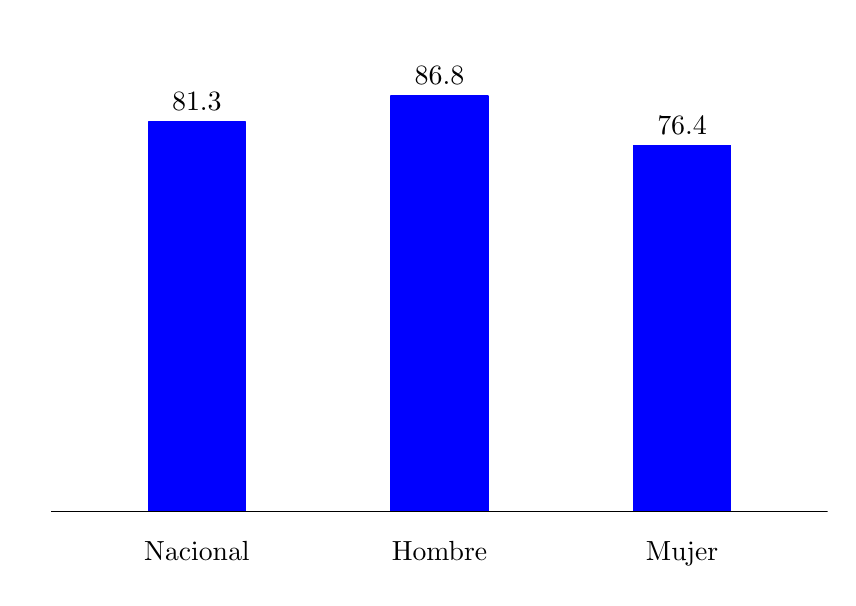
\begin{tikzpicture}[x=1pt,y=1pt]  % Created by tikzDevice version 0.9 on 2015-12-11 10:47:30
% !TEX encoding = UTF-8 Unicode
\definecolor{fillColor}{RGB}{255,255,255}
\path[use as bounding box,fill=fillColor,fill opacity=0.00] (0,0) rectangle (289.08,198.74);
\begin{scope}
\path[clip] (  0.00,  0.00) rectangle (289.08,198.74);

\path[] (  0.00,  0.00) rectangle (289.08,198.74);
\end{scope}
\begin{scope}
\path[clip] (  0.00,  0.00) rectangle (289.08,198.74);

\path[] (  8.54, 16.35) rectangle (289.08,181.67);

\path[] ( 61.14, 16.35) --
	( 61.14,181.67);

\path[] (148.81, 16.35) --
	(148.81,181.67);

\path[] (236.48, 16.35) --
	(236.48,181.67);
\definecolor{drawColor}{RGB}{0,0,255}
\definecolor{fillColor}{RGB}{0,0,255}

\path[draw=drawColor,line width= 0.6pt,line join=round,fill=fillColor] ( 43.60, 23.87) rectangle ( 78.67,164.68);

\path[draw=drawColor,line width= 0.6pt,line join=round,fill=fillColor] (131.27, 23.87) rectangle (166.34,174.16);

\path[draw=drawColor,line width= 0.6pt,line join=round,fill=fillColor] (218.94, 23.87) rectangle (254.01,156.17);
\definecolor{drawColor}{RGB}{0,0,0}

\path[draw=drawColor,line width= 0.1pt,line join=round] (  8.54, 23.87) -- (289.08, 23.87);

\node[text=drawColor,anchor=base,inner sep=0pt, outer sep=0pt, scale=  1.01] at ( 61.14,168.64) {81.3};

\node[text=drawColor,anchor=base,inner sep=0pt, outer sep=0pt, scale=  1.01] at (148.81,178.11) {86.8};

\node[text=drawColor,anchor=base,inner sep=0pt, outer sep=0pt, scale=  1.01] at (236.48,160.12) {76.4};

\path[] (  8.54, 16.35) rectangle (289.08,181.67);
\end{scope}
\begin{scope}
\path[clip] (  0.00,  0.00) rectangle (289.08,198.74);

\path[] (  8.54, 16.35) --
	(  8.54,181.67);
\end{scope}
\begin{scope}
\path[clip] (  0.00,  0.00) rectangle (289.08,198.74);

\path[] (  8.54, 16.35) --
	(289.08, 16.35);
\end{scope}
\begin{scope}
\path[clip] (  0.00,  0.00) rectangle (289.08,198.74);

\path[] ( 61.14, 12.08) --
	( 61.14, 16.35);

\path[] (148.81, 12.08) --
	(148.81, 16.35);

\path[] (236.48, 12.08) --
	(236.48, 16.35);
\end{scope}
\begin{scope}
\path[clip] (  0.00,  0.00) rectangle (289.08,198.74);
\definecolor{drawColor}{RGB}{0,0,0}

\node[text=drawColor,anchor=base,inner sep=0pt, outer sep=0pt, scale=  1.00] at ( 61.14,  6.04) {Nacional};

\node[text=drawColor,anchor=base,inner sep=0pt, outer sep=0pt, scale=  1.00] at (148.81,  6.04) {Hombre};

\node[text=drawColor,anchor=base,inner sep=0pt, outer sep=0pt, scale=  1.00] at (236.48,  6.04) {Mujer};
\end{scope}
  \end{tikzpicture}}{Instituto Nacional de Estadística, con datos de Enei II-2014}

\cajita{Alfabetismo por edad}{Según la desagregación de la población en edad de trabajar por grandes grupos de edad, el 91\% de la población joven (comprendidos entre los 15 y 29 años) sabe leer y escribir, siendo este el grupo que presenta la mayor tasa de alfabetismo. Los adultos entre los 30 y 54 años presentan una tasa de alfabetismo del 71.3\%.}{Tasa de alfabetismo en personas mayores de 14 años\\ por grupo etario}{República de Guatemala, año 2014, en porcentaje}{\ \\[0mm]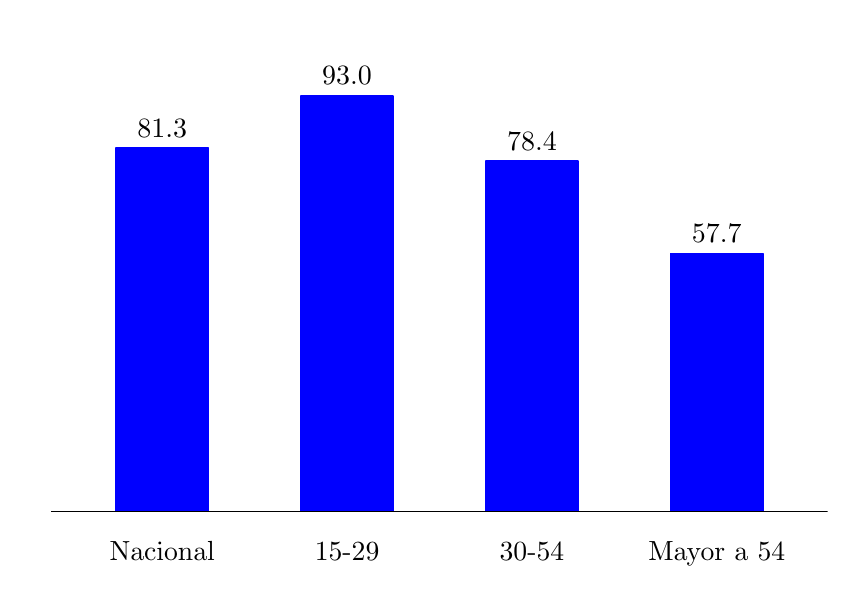
\begin{tikzpicture}[x=1pt,y=1pt]  % Created by tikzDevice version 0.9 on 2015-12-11 10:47:30
% !TEX encoding = UTF-8 Unicode
\definecolor{fillColor}{RGB}{255,255,255}
\path[use as bounding box,fill=fillColor,fill opacity=0.00] (0,0) rectangle (289.08,198.74);
\begin{scope}
\path[clip] (  0.00,  0.00) rectangle (289.08,198.74);

\path[] (  0.00,  0.00) rectangle (289.08,198.74);
\end{scope}
\begin{scope}
\path[clip] (  0.00,  0.00) rectangle (289.08,198.74);

\path[] (  8.54, 16.35) rectangle (289.08,181.67);

\path[] ( 48.61, 16.35) --
	( 48.61,181.67);

\path[] (115.41, 16.35) --
	(115.41,181.67);

\path[] (182.21, 16.35) --
	(182.21,181.67);

\path[] (249.00, 16.35) --
	(249.00,181.67);
\definecolor{drawColor}{RGB}{0,0,255}
\definecolor{fillColor}{RGB}{0,0,255}

\path[draw=drawColor,line width= 0.6pt,line join=round,fill=fillColor] ( 31.91, 23.87) rectangle ( 65.31,155.18);

\path[draw=drawColor,line width= 0.6pt,line join=round,fill=fillColor] ( 98.71, 23.87) rectangle (132.11,174.16);

\path[draw=drawColor,line width= 0.6pt,line join=round,fill=fillColor] (165.51, 23.87) rectangle (198.91,150.50);

\path[draw=drawColor,line width= 0.6pt,line join=round,fill=fillColor] (232.30, 23.87) rectangle (265.70,117.12);
\definecolor{drawColor}{RGB}{0,0,0}

\path[draw=drawColor,line width= 0.1pt,line join=round] (  8.54, 23.87) -- (289.08, 23.87);

\node[text=drawColor,anchor=base,inner sep=0pt, outer sep=0pt, scale=  1.01] at ( 48.61,159.13) {81.3};

\node[text=drawColor,anchor=base,inner sep=0pt, outer sep=0pt, scale=  1.01] at (115.41,178.11) {93.0};

\node[text=drawColor,anchor=base,inner sep=0pt, outer sep=0pt, scale=  1.01] at (182.21,154.46) {78.4};

\node[text=drawColor,anchor=base,inner sep=0pt, outer sep=0pt, scale=  1.01] at (249.00,121.07) {57.7};

\path[] (  8.54, 16.35) rectangle (289.08,181.67);
\end{scope}
\begin{scope}
\path[clip] (  0.00,  0.00) rectangle (289.08,198.74);

\path[] (  8.54, 16.35) --
	(  8.54,181.67);
\end{scope}
\begin{scope}
\path[clip] (  0.00,  0.00) rectangle (289.08,198.74);

\path[] (  8.54, 16.35) --
	(289.08, 16.35);
\end{scope}
\begin{scope}
\path[clip] (  0.00,  0.00) rectangle (289.08,198.74);

\path[] ( 48.61, 12.08) --
	( 48.61, 16.35);

\path[] (115.41, 12.08) --
	(115.41, 16.35);

\path[] (182.21, 12.08) --
	(182.21, 16.35);

\path[] (249.00, 12.08) --
	(249.00, 16.35);
\end{scope}
\begin{scope}
\path[clip] (  0.00,  0.00) rectangle (289.08,198.74);
\definecolor{drawColor}{RGB}{0,0,0}

\node[text=drawColor,anchor=base,inner sep=0pt, outer sep=0pt, scale=  1.00] at ( 48.61,  6.04) {Nacional};

\node[text=drawColor,anchor=base,inner sep=0pt, outer sep=0pt, scale=  1.00] at (115.41,  6.04) {15-29};

\node[text=drawColor,anchor=base,inner sep=0pt, outer sep=0pt, scale=  1.00] at (182.21,  6.04) {30-54};

\node[text=drawColor,anchor=base,inner sep=0pt, outer sep=0pt, scale=  1.00] at (249.00,  6.04) {Mayor a 54};
\end{scope}
  \end{tikzpicture}}{Instituto Nacional de Estadística, con datos de Enei II-2014}

\cajita{Alfabetismo por etnia}{Con la desagregación de la tasa de alfabetismo de las personas en edad de trabajar según su grupo étnico, se muestra que las personas no indígenas presentan la tasa mayor de alfabetismo (83.8\%) comparada con la de la población indígena (64.1\%) ,indica que la tasa de analfabetismo es 2.2 veces mayor en la población indígena.}{Tasa de alfabetismo en personas mayores\\ de 14 años por grupo étnico}{República de Guatemala, año 2014, en porcentaje}{\ \\[0mm]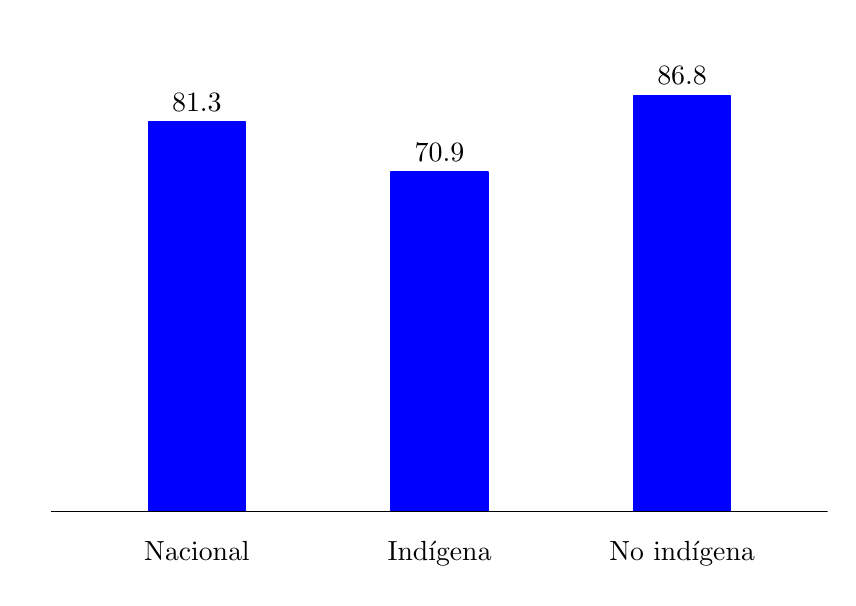
\begin{tikzpicture}[x=1pt,y=1pt]  % Created by tikzDevice version 0.9 on 2015-12-11 10:47:31
% !TEX encoding = UTF-8 Unicode
\definecolor{fillColor}{RGB}{255,255,255}
\path[use as bounding box,fill=fillColor,fill opacity=0.00] (0,0) rectangle (289.08,198.74);
\begin{scope}
\path[clip] (  0.00,  0.00) rectangle (289.08,198.74);

\path[] (  0.00,  0.00) rectangle (289.08,198.74);
\end{scope}
\begin{scope}
\path[clip] (  0.00,  0.00) rectangle (289.08,198.74);

\path[] (  8.54, 16.35) rectangle (289.08,181.67);

\path[] ( 61.14, 16.35) --
	( 61.14,181.67);

\path[] (148.81, 16.35) --
	(148.81,181.67);

\path[] (236.48, 16.35) --
	(236.48,181.67);
\definecolor{drawColor}{RGB}{0,0,255}
\definecolor{fillColor}{RGB}{0,0,255}

\path[draw=drawColor,line width= 0.6pt,line join=round,fill=fillColor] ( 43.60, 23.87) rectangle ( 78.67,164.55);

\path[draw=drawColor,line width= 0.6pt,line join=round,fill=fillColor] (131.27, 23.87) rectangle (166.34,146.55);

\path[draw=drawColor,line width= 0.6pt,line join=round,fill=fillColor] (218.94, 23.87) rectangle (254.01,174.16);
\definecolor{drawColor}{RGB}{0,0,0}

\path[draw=drawColor,line width= 0.1pt,line join=round] (  8.54, 23.87) -- (289.08, 23.87);

\node[text=drawColor,anchor=base,inner sep=0pt, outer sep=0pt, scale=  1.01] at ( 61.14,168.51) {81.3};

\node[text=drawColor,anchor=base,inner sep=0pt, outer sep=0pt, scale=  1.01] at (148.81,150.51) {70.9};

\node[text=drawColor,anchor=base,inner sep=0pt, outer sep=0pt, scale=  1.01] at (236.48,178.11) {86.8};

\path[] (  8.54, 16.35) rectangle (289.08,181.67);
\end{scope}
\begin{scope}
\path[clip] (  0.00,  0.00) rectangle (289.08,198.74);

\path[] (  8.54, 16.35) --
	(  8.54,181.67);
\end{scope}
\begin{scope}
\path[clip] (  0.00,  0.00) rectangle (289.08,198.74);

\path[] (  8.54, 16.35) --
	(289.08, 16.35);
\end{scope}
\begin{scope}
\path[clip] (  0.00,  0.00) rectangle (289.08,198.74);

\path[] ( 61.14, 12.08) --
	( 61.14, 16.35);

\path[] (148.81, 12.08) --
	(148.81, 16.35);

\path[] (236.48, 12.08) --
	(236.48, 16.35);
\end{scope}
\begin{scope}
\path[clip] (  0.00,  0.00) rectangle (289.08,198.74);
\definecolor{drawColor}{RGB}{0,0,0}

\node[text=drawColor,anchor=base,inner sep=0pt, outer sep=0pt, scale=  1.00] at ( 61.14,  6.04) {Nacional};

\node[text=drawColor,anchor=base,inner sep=0pt, outer sep=0pt, scale=  1.00] at (148.81,  6.04) {Indígena};

\node[text=drawColor,anchor=base,inner sep=0pt, outer sep=0pt, scale=  1.00] at (236.48,  6.04) {No indígena};
\end{scope}
  \end{tikzpicture}}{Instituto Nacional de Estadística, con datos de Enei II-2014}

\cajita{Alfabetismo según etnia y sexo}{La tasas de alfabetismo en las personas mayores de 14 años, desagregada por etnia y sexo, muestra que los hombres  no indígenas tienen la mayor tasa de alfabetismo con el 85.6\%, quienes presentan una diferencia de 11.4 puntos porcentuales respecto a los hombres indígenas.  La menor tasa la presentan las mujeres indígenas con un 55.0\%.}{Tasa de alfabetismo  en personas mayores de 14 años \\ según etnia y  sexo}{República de Guatemala, año 2014, en porcentaje}{\ \\[0mm]\begin{tikzpicture}[x=1pt,y=1pt]  % Created by tikzDevice version 0.9 on 2015-12-11 10:47:31
% !TEX encoding = UTF-8 Unicode
\definecolor{fillColor}{RGB}{255,255,255}
\path[use as bounding box,fill=fillColor,fill opacity=0.00] (0,0) rectangle (289.08,198.74);
\begin{scope}
\path[clip] (  0.00,  0.00) rectangle (289.08,198.74);

\path[] (  0.00,  0.00) rectangle (289.08,198.74);
\end{scope}
\begin{scope}
\path[clip] (  0.00,  0.00) rectangle (289.08,198.74);

\path[] (  7.11, 20.62) rectangle (289.08,172.85);

\path[] ( 84.01, 20.62) --
	( 84.01,172.85);

\path[] (212.18, 20.62) --
	(212.18,172.85);
\definecolor{drawColor}{RGB}{0,0,255}
\definecolor{fillColor}{RGB}{0,0,255}

\path[draw=drawColor,line width= 0.6pt,line join=round,fill=fillColor] ( 34.35, 20.62) rectangle ( 76.00,156.00);
\definecolor{drawColor}{RGB}{157,187,255}
\definecolor{fillColor}{RGB}{157,187,255}

\path[draw=drawColor,line width= 0.6pt,line join=round,fill=fillColor] ( 92.02, 20.62) rectangle (133.68,126.26);
\definecolor{drawColor}{RGB}{0,0,255}
\definecolor{fillColor}{RGB}{0,0,255}

\path[draw=drawColor,line width= 0.6pt,line join=round,fill=fillColor] (162.52, 20.62) rectangle (204.17,172.85);
\definecolor{drawColor}{RGB}{157,187,255}
\definecolor{fillColor}{RGB}{157,187,255}

\path[draw=drawColor,line width= 0.6pt,line join=round,fill=fillColor] (220.19, 20.62) rectangle (261.84,162.02);
\definecolor{drawColor}{RGB}{0,0,0}

\path[draw=drawColor,line width= 0.6pt,line join=round] (  7.11, 20.62) -- (289.08, 20.62);

\node[text=drawColor,anchor=base,inner sep=0pt, outer sep=0pt, scale=  0.82] at ( 55.18,159.23) {80.2};

\node[text=drawColor,anchor=base,inner sep=0pt, outer sep=0pt, scale=  0.82] at (112.85,129.48) {62.6};

\node[text=drawColor,anchor=base,inner sep=0pt, outer sep=0pt, scale=  0.82] at (183.34,176.07) {90.2};

\node[text=drawColor,anchor=base,inner sep=0pt, outer sep=0pt, scale=  0.82] at (241.02,165.24) {83.8};

\path[] (  7.11, 20.62) rectangle (289.08,172.85);
\end{scope}
\begin{scope}
\path[clip] (  0.00,  0.00) rectangle (289.08,198.74);

\path[] (  7.11, 20.62) --
	(  7.11,172.85);
\end{scope}
\begin{scope}
\path[clip] (  0.00,  0.00) rectangle (289.08,198.74);

\path[] (  7.11, 20.62) --
	(289.08, 20.62);
\end{scope}
\begin{scope}
\path[clip] (  0.00,  0.00) rectangle (289.08,198.74);

\path[] ( 84.01, 16.35) --
	( 84.01, 20.62);

\path[] (212.18, 16.35) --
	(212.18, 20.62);
\end{scope}
\begin{scope}
\path[clip] (  0.00,  0.00) rectangle (289.08,198.74);
\definecolor{drawColor}{RGB}{0,0,0}

\node[text=drawColor,anchor=base,inner sep=0pt, outer sep=0pt, scale=  1.00] at ( 84.01,  5.69) {Indígena};

\node[text=drawColor,anchor=base,inner sep=0pt, outer sep=0pt, scale=  1.00] at (212.18,  5.69) {No indígena};
\end{scope}
\begin{scope}
\path[clip] (  0.00,  0.00) rectangle (289.08,198.74);
\coordinate (apoyo) at (55.98,189.21);
\coordinate (longitudFicticia) at (7.11,9.53);
\coordinate (longitud) at (7.11,7.11);
\coordinate (desX) at (142.21,0);
\coordinate (desY) at (0,1.21);
\definecolor[named]{ct1}{HTML}{
0000FF
}
\definecolor[named]{ct2}{HTML}{
9DBBFF
}
\definecolor[named]{ctb1}{HTML}{
0000FF
}
\definecolor[named]{ctb2}{HTML}{
9DBBFF
}
\path [fill=none] (apoyo) rectangle ($(apoyo)+(longitudFicticia)$)
node [xshift=0.3cm,inner sep=0pt, outer sep=0pt,midway,right,scale = 0.9]{Hombre};
\draw [color = ctb1,fill=ct1] ( $(apoyo)  + (desY) $) rectangle ($(apoyo)+ (desY) +(longitud)$);
\path [fill=none] ($(apoyo)+(desX)$) rectangle ($(apoyo)+(desX)+(longitudFicticia)$)
node [xshift=0.3cm,inner sep=0pt, outer sep=0pt,midway,right,scale = 0.9]{Mujer};
\draw [color = ctb2 ,fill=ct2] ( $(apoyo)  + (desY) + (desX) $) rectangle ($(apoyo)+ (desY)+ (desX) +(longitud)$);
\end{scope}
  \end{tikzpicture}}{Instituto Nacional de Estadística, con datos de Enei II-2014}

\cajita{Alfabetismo por área de residencia}{Las personas en edad de trabajar presentandiferencias en la tasa de alfabetismo, al realizar una desagregación según el área de residencia, siendo esta mayor en el área urbana con el 82.9\%, que en el área rural, teniendo una diferencia de 14.9 puntos porcentuales.}{Tasa de alfabetismo en personas mayores de 14 años por área}{República de Guatemala, año 2014, en porcentaje}{\ \\[0mm]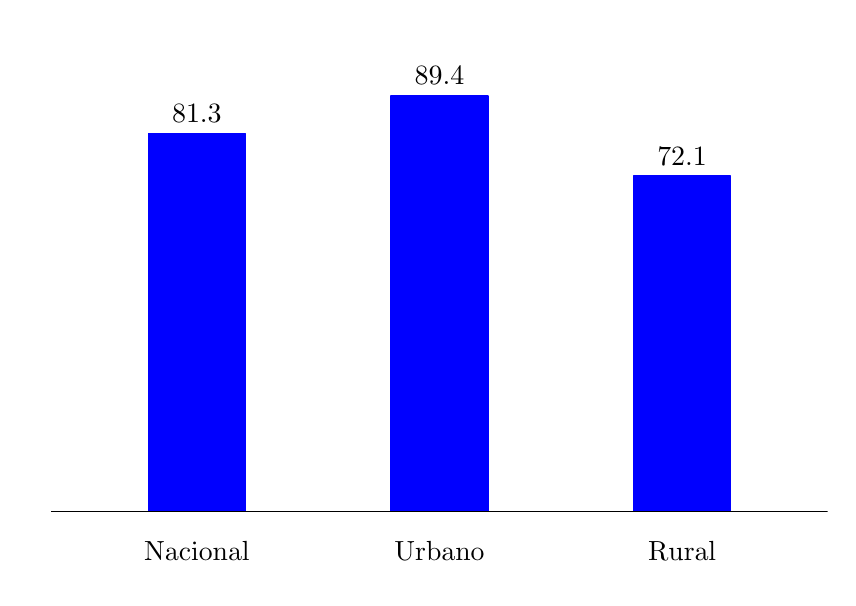
\begin{tikzpicture}[x=1pt,y=1pt]  % Created by tikzDevice version 0.9 on 2015-12-11 10:47:33
% !TEX encoding = UTF-8 Unicode
\definecolor{fillColor}{RGB}{255,255,255}
\path[use as bounding box,fill=fillColor,fill opacity=0.00] (0,0) rectangle (289.08,198.74);
\begin{scope}
\path[clip] (  0.00,  0.00) rectangle (289.08,198.74);

\path[] (  0.00,  0.00) rectangle (289.08,198.74);
\end{scope}
\begin{scope}
\path[clip] (  0.00,  0.00) rectangle (289.08,198.74);

\path[] (  8.54, 16.35) rectangle (289.08,181.67);

\path[] ( 61.14, 16.35) --
	( 61.14,181.67);

\path[] (148.81, 16.35) --
	(148.81,181.67);

\path[] (236.48, 16.35) --
	(236.48,181.67);
\definecolor{drawColor}{RGB}{0,0,255}
\definecolor{fillColor}{RGB}{0,0,255}

\path[draw=drawColor,line width= 0.6pt,line join=round,fill=fillColor] ( 43.60, 23.87) rectangle ( 78.67,160.49);

\path[draw=drawColor,line width= 0.6pt,line join=round,fill=fillColor] (131.27, 23.87) rectangle (166.34,174.16);

\path[draw=drawColor,line width= 0.6pt,line join=round,fill=fillColor] (218.94, 23.87) rectangle (254.01,145.04);
\definecolor{drawColor}{RGB}{0,0,0}

\path[draw=drawColor,line width= 0.1pt,line join=round] (  8.54, 23.87) -- (289.08, 23.87);

\node[text=drawColor,anchor=base,inner sep=0pt, outer sep=0pt, scale=  1.01] at ( 61.14,164.44) {81.3};

\node[text=drawColor,anchor=base,inner sep=0pt, outer sep=0pt, scale=  1.01] at (148.81,178.11) {89.4};

\node[text=drawColor,anchor=base,inner sep=0pt, outer sep=0pt, scale=  1.01] at (236.48,148.99) {72.1};

\path[] (  8.54, 16.35) rectangle (289.08,181.67);
\end{scope}
\begin{scope}
\path[clip] (  0.00,  0.00) rectangle (289.08,198.74);

\path[] (  8.54, 16.35) --
	(  8.54,181.67);
\end{scope}
\begin{scope}
\path[clip] (  0.00,  0.00) rectangle (289.08,198.74);

\path[] (  8.54, 16.35) --
	(289.08, 16.35);
\end{scope}
\begin{scope}
\path[clip] (  0.00,  0.00) rectangle (289.08,198.74);

\path[] ( 61.14, 12.08) --
	( 61.14, 16.35);

\path[] (148.81, 12.08) --
	(148.81, 16.35);

\path[] (236.48, 12.08) --
	(236.48, 16.35);
\end{scope}
\begin{scope}
\path[clip] (  0.00,  0.00) rectangle (289.08,198.74);
\definecolor{drawColor}{RGB}{0,0,0}

\node[text=drawColor,anchor=base,inner sep=0pt, outer sep=0pt, scale=  1.00] at ( 61.14,  6.04) {Nacional};

\node[text=drawColor,anchor=base,inner sep=0pt, outer sep=0pt, scale=  1.00] at (148.81,  6.04) {Urbano};

\node[text=drawColor,anchor=base,inner sep=0pt, outer sep=0pt, scale=  1.00] at (236.48,  6.04) {Rural};
\end{scope}
  \end{tikzpicture}}{Instituto Nacional de Estadística, con datos de Enei II-2014}

\cajita{Alfabetismo por área y sexo}{La tasas de alfabetismo en las personas mayores de 14 años, desagregada por área de residencia (urbano – rural) y sexo, muestra que los hombres  del área urbana tienen la mayor tasa de alfabetismo con el 87.3\%, con una diferencia de 13.2 puntos porcentuales respecto a los hombres del área rural, esto es que la tasa de analfabetismo en hombres rurales es 2.0 veces mayor que la de los hombres urbanos.
	
	 La menor tasa de alfabetismo la presentan las mujeres rurales,  con un 62.6\%.}{Tasa de alfabetismo en personas mayores de 14 años\\ por área y sexo}{República de Guatemala, año 2014, en porcentaje}{\ \\[0mm]\begin{tikzpicture}[x=1pt,y=1pt]  % Created by tikzDevice version 0.9 on 2015-12-11 10:47:33
% !TEX encoding = UTF-8 Unicode
\definecolor{fillColor}{RGB}{255,255,255}
\path[use as bounding box,fill=fillColor,fill opacity=0.00] (0,0) rectangle (289.08,198.74);
\begin{scope}
\path[clip] (  0.00,  0.00) rectangle (289.08,198.74);

\path[] (  0.00,  0.00) rectangle (289.08,198.74);
\end{scope}
\begin{scope}
\path[clip] (  0.00,  0.00) rectangle (289.08,198.74);

\path[] (  7.11, 20.62) rectangle (289.08,172.85);

\path[] ( 84.01, 20.62) --
	( 84.01,172.85);

\path[] (212.18, 20.62) --
	(212.18,172.85);
\definecolor{drawColor}{RGB}{0,0,255}
\definecolor{fillColor}{RGB}{0,0,255}

\path[draw=drawColor,line width= 0.6pt,line join=round,fill=fillColor] ( 34.35, 20.62) rectangle ( 76.00,172.85);
\definecolor{drawColor}{RGB}{157,187,255}
\definecolor{fillColor}{RGB}{157,187,255}

\path[draw=drawColor,line width= 0.6pt,line join=round,fill=fillColor] ( 92.02, 20.62) rectangle (133.68,159.77);
\definecolor{drawColor}{RGB}{0,0,255}
\definecolor{fillColor}{RGB}{0,0,255}

\path[draw=drawColor,line width= 0.6pt,line join=round,fill=fillColor] (162.52, 20.62) rectangle (204.17,149.16);
\definecolor{drawColor}{RGB}{157,187,255}
\definecolor{fillColor}{RGB}{157,187,255}

\path[draw=drawColor,line width= 0.6pt,line join=round,fill=fillColor] (220.19, 20.62) rectangle (261.84,127.13);
\definecolor{drawColor}{RGB}{0,0,0}

\path[draw=drawColor,line width= 0.6pt,line join=round] (  7.11, 20.62) -- (289.08, 20.62);

\node[text=drawColor,anchor=base,inner sep=0pt, outer sep=0pt, scale=  0.82] at ( 55.18,176.07) {93.7};

\node[text=drawColor,anchor=base,inner sep=0pt, outer sep=0pt, scale=  0.82] at (112.85,162.99) {85.7};

\node[text=drawColor,anchor=base,inner sep=0pt, outer sep=0pt, scale=  0.82] at (183.34,152.38) {79.1};

\node[text=drawColor,anchor=base,inner sep=0pt, outer sep=0pt, scale=  0.82] at (241.02,130.36) {65.6};

\path[] (  7.11, 20.62) rectangle (289.08,172.85);
\end{scope}
\begin{scope}
\path[clip] (  0.00,  0.00) rectangle (289.08,198.74);

\path[] (  7.11, 20.62) --
	(  7.11,172.85);
\end{scope}
\begin{scope}
\path[clip] (  0.00,  0.00) rectangle (289.08,198.74);

\path[] (  7.11, 20.62) --
	(289.08, 20.62);
\end{scope}
\begin{scope}
\path[clip] (  0.00,  0.00) rectangle (289.08,198.74);

\path[] ( 84.01, 16.35) --
	( 84.01, 20.62);

\path[] (212.18, 16.35) --
	(212.18, 20.62);
\end{scope}
\begin{scope}
\path[clip] (  0.00,  0.00) rectangle (289.08,198.74);
\definecolor{drawColor}{RGB}{0,0,0}

\node[text=drawColor,anchor=base,inner sep=0pt, outer sep=0pt, scale=  1.00] at ( 84.01,  5.69) {Urbano};

\node[text=drawColor,anchor=base,inner sep=0pt, outer sep=0pt, scale=  1.00] at (212.18,  5.69) {Rural};
\end{scope}
\begin{scope}
\path[clip] (  0.00,  0.00) rectangle (289.08,198.74);
\coordinate (apoyo) at (55.98,189.21);
\coordinate (longitudFicticia) at (7.11,9.53);
\coordinate (longitud) at (7.11,7.11);
\coordinate (desX) at (142.21,0);
\coordinate (desY) at (0,1.21);
\definecolor[named]{ct1}{HTML}{
0000FF
}
\definecolor[named]{ct2}{HTML}{
9DBBFF
}
\definecolor[named]{ctb1}{HTML}{
0000FF
}
\definecolor[named]{ctb2}{HTML}{
9DBBFF
}
\path [fill=none] (apoyo) rectangle ($(apoyo)+(longitudFicticia)$)
node [xshift=0.3cm,inner sep=0pt, outer sep=0pt,midway,right,scale = 0.9]{Hombre};
\draw [color = ctb1,fill=ct1] ( $(apoyo)  + (desY) $) rectangle ($(apoyo)+ (desY) +(longitud)$);
\path [fill=none] ($(apoyo)+(desX)$) rectangle ($(apoyo)+(desX)+(longitudFicticia)$)
node [xshift=0.3cm,inner sep=0pt, outer sep=0pt,midway,right,scale = 0.9]{Mujer};
\draw [color = ctb2 ,fill=ct2] ( $(apoyo)  + (desY) + (desX) $) rectangle ($(apoyo)+ (desY)+ (desX) +(longitud)$);
\end{scope}
  \end{tikzpicture}}{Instituto Nacional de Estadística, con datos de Enei II-2014}


